\documentclass{article}
\usepackage[utf8]{vietnam}
\usepackage{graphicx}
\usepackage{amsmath}
\usepackage{amssymb}
\usepackage{hyperref}
\usepackage{caption}
\usepackage{subcaption}

\title{Image Restoration\\ \Large Report Lab Week 5-6 Part2}
\author{Ngọc Thuận - IPSAL LAB}
\date{December 2022}

\begin{document}
\maketitle
\begin{abstract}
    Ta đã đi qua cơ bản về các phép lọc để xử lí ảnh số, mục đích đơn giản nhất đó là ứng dụng các phép lọc đã biết, kết hợp với các kiến thức toán học để giải quyết các bài toán liên quan đến ảnh chất lượng kém. Trong bài này ta sẽ điểm qua một vài phép khôi phục ảnh nổi bật!
\end{abstract}

\section{Introduction}
    \subsection{Khôi phục ảnh là gì? - What is image restoration?}
    Trước hết ta cần phân biệt \textit{Khôi phục ảnh} và \textit{Tăng cường ảnh}. Điểm khác biệt cơ bản ở đây là \textit{Khôi phục ảnh} khách quan hơn, \textit{Tăng cường ảnh} sẽ chủ quan hơn.\\
    \textit{Khôi phục ảnh} chỉ đơn giản là đi xác định quá trình xuống cấp, và cố gắng khôi phục nó!
    \subsection{Các mô hình nhiễu}
    Có thể nói nguồn gốc của nhiễu trong ảnh kĩ thuật số có thể xuất hiện trong quá trình thu thập và truyền đạt hình ảnh:
    \begin{enumerate}
        \item Có thể do cảm biến bị ảnh hưởng bởi mỗi trường xung quanh.
        \item Cũng có thể có sự tác động từ bên ngoài trong quá trình truyền đạt ảnh.
        \item vân vân \ldots
    \end{enumerate}
    Cơ bản, một bức ảnh nhiễu có thể được \textit{model} hóa như sau:
    $$g(x,y) = f(x,y) + \eta (x,y)$$
    trong đó:
    \begin{itemize}
        \item $f(x,y)$ là ảnh gốc.
        \item $\eta (x,y)$ là nhiễu
        \item $g(x,y)$ là kết quả - ảnh nhiễu
    \end{itemize}
    Việc xác định được \textit{model} của nhiễu giúp ta xác định được các cách giải quyết khi gặp nhiễu!\\
    \subsubsection*{Một số mô hình nhiễu cơ bản}
    \begin{figure}[ht!]
        \centering
        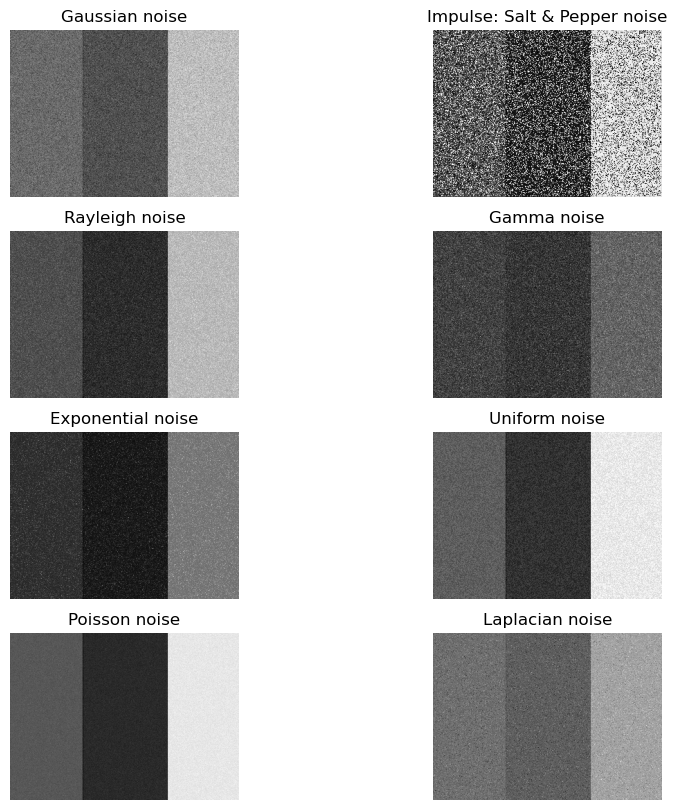
\includegraphics[width = \linewidth]{n1.png}
        \caption{Một số nhiễu cơ bản}
        \label{fig1}
    \end{figure}
    Hình \ref{fig1} cho ta một số mỗ hình nhiều cơ bản.
    \begin{figure}[ht!]
        \centering
        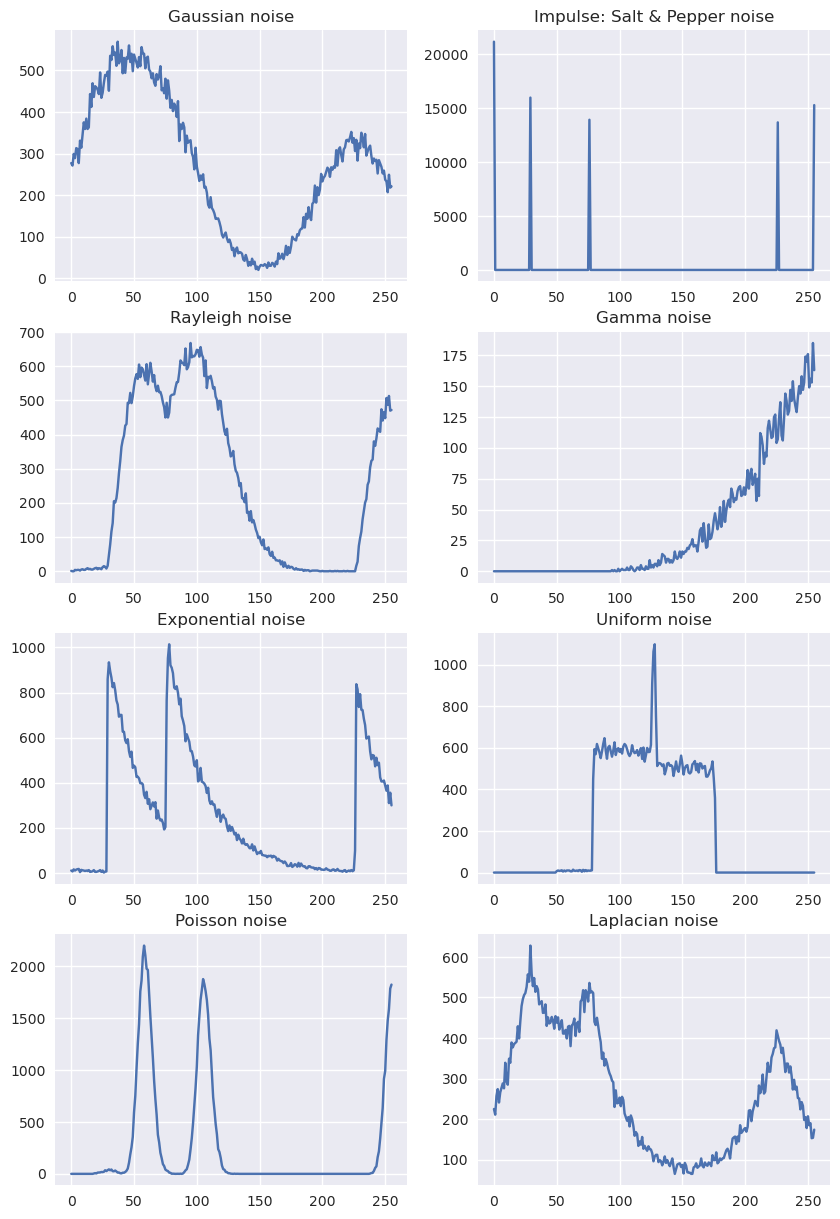
\includegraphics[width = \linewidth]{n2.png}
        \caption{Lược đồ xám của một số mô hình nhiễu cơ bản}
        \label{fig2}
    \end{figure}
    \\ \\ Hình \ref{fig2} cho ta lược đồ xám của chúng!
    \subsubsection*{Nhiễu tuần hoàn}
    Nhiễu tuần hoàn có thể biểu diễn như sau:\\
    \underline{Trong miền không gian}
    $$r(x,y) = A \sin \left[2\pi u_0 (x+B_x)/M + 2\pi v_0 (y+ B_y) /N \right]$$
    Trong đó, $A$ là biên độ, $u_0, v_0$ là tần số, $B_x B_y$ là độ lệch pha.\\
    \underline{Trong miền tần số}
    $$R(u,v) = j\frac{AMN}{2} \left[ e^{-j2\pi(u_0B_x/M+v_0B_y/N}\delta(u+u_0,v+v_0)-e^{j2\pi(u_0B_x/M+v_0B_y/N)}\delta(u-u_0,v-v_0) \right]$$
    \begin{figure}[ht!]
        \centering
        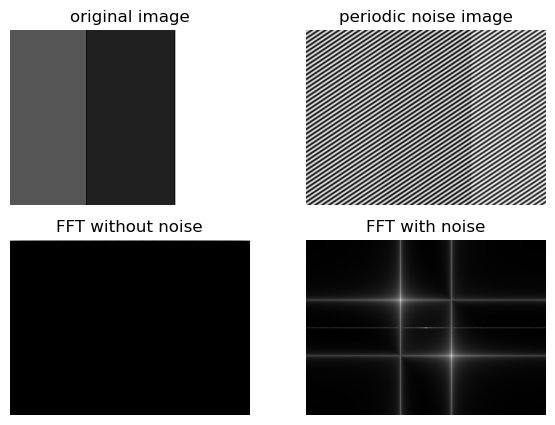
\includegraphics[width = \linewidth]{n3.png}
        \caption{Nhiễu tuần hoàn}
        \label{fig3}
    \end{figure}
    \sectiion{Addtive Random Noise Reduction}
    \subsection{Mean Filter}
\end{document}
